\documentclass[11pt,a4paper]{article}

\usepackage[margin=2.1cm]{geometry}
\usepackage[T1]{fontenc}
\usepackage{lmodern}
\usepackage{microtype}
\usepackage{amsmath}
\usepackage{booktabs}
\usepackage{array}
\usepackage{xcolor}
\usepackage{graphicx}
\usepackage{float}
\usepackage{listings}
\usepackage[hidelinks]{hyperref}

\graphicspath{{../lab/lab3/task1/}{../lab/lab3/task2/}}

\definecolor{codebg}{RGB}{246,248,250}
\definecolor{coderule}{RGB}{208,215,222}
\lstset{
  basicstyle=\ttfamily\small,
  backgroundcolor=\color{codebg},
  frame=single,
  rulecolor=\color{coderule},
  breaklines=true,
  columns=fullflexible,
  keepspaces=true,
  showstringspaces=false,
  xleftmargin=0.3em,
  xrightmargin=0.3em
}
\newcommand{\code}[1]{\texttt{#1}}

\title{\textbf{Lab 3 Report: Topology and Flow Control}\\[0.4em]
       \large gem5 Garnet Network-on-Chip Simulation}
\author{\begin{tabular}{rl}
          Name: & \rule{7cm}{0.4pt} \\
          Student ID: & \rule{7cm}{0.4pt}
        \end{tabular}}
\date{gem5 v23.0.0.1 \quad July 2026}

\begin{document}
\maketitle

\begin{abstract}
This laboratory extends Garnet with a 16-node bidirectional Ring topology,
custom shortest-path routing, and a wormhole-style flow-control mode for
single-flit control traffic. Ring and 4x4 Mesh experiments are swept over 50
injection rates. A second sweep compares one VC of depth one, sixteen VCs of
depth one, and one wormhole VC of depth sixteen. The Ring has a low-load
latency of 13.158 Ruby cycles and reaches a stable throughput of 0.233756
packets/node/Ruby cycle before the finite-window experiment shows blocking.
The two 16-slot alternatives sustain approximately 0.248 packets/node/Ruby
cycle across the tested range, while the one-slot baseline stalls at 0.09
injection rate.
\end{abstract}

\tableofcontents
\newpage

\section{Experimental Method}

Experiments use gem5 v23.0.0.1, the NULL ISA, and the
\code{Garnet\_standalone} protocol. The global frequency is 2 GHz, so one
Ruby tick is 0.5 ns. Each run lasts 10000 Ruby cycles, equivalent to 5000
system cycles because the synthetic traffic generator uses a 1 GHz system
clock. Injection rates are specified in packets/node/system-cycle; the
corresponding offered load per Ruby cycle is

\begin{equation}
  \lambda_{Ruby}=\frac{\lambda_{system}}{2}.
\end{equation}

For received packet count $N_r$, the reported throughput is

\begin{equation}
  T=\frac{N_r}{N_{nodes}\,10000}.
\end{equation}

Both tasks use vnet 0, which carries single-flit control packets and uniform
random destinations. A point is called \emph{stalled} when source injection
acceptance is below 0.9 of the expected Bernoulli-generated packet count. This
indicates backpressure or a cyclic congestion condition in the finite run; it
does not mean that the gem5 process crashed.

\section{Task 1: Ring Topology}

\subsection{Implementation}

\code{configs/topologies/Ring.py} constructs exactly 16 routers, one external
link per router, and two directed internal links per router. The two ports are
named \code{Clockwise} and \code{CounterClockwise}. The custom routing method
in \code{RoutingUnit::outportComputeCustom()} computes clockwise and
counter-clockwise modular distances and selects the shorter direction; ties
are resolved clockwise. Thus packets use shortest paths on the physical
bidirectional ring.

The relevant build command is:

\begin{lstlisting}[language=bash]
scons --ignore-style build/NULL/gem5.opt \\
  PROTOCOL=Garnet_standalone -j$(nproc)
\end{lstlisting}

Directed smoke tests verified one-hop paths for 0 to 15 and 15 to 0, an
eight-hop antipodal path for 0 to 8, and a five-hop path for 3 to 14.

\subsection{Measured comparison}

The sweep contains 50 rates from 0.01 through 0.50 for both the Ring and a
4x4 Mesh with the same 16 nodes.

\begin{table}[H]
\centering
\small
\caption{Task 1 summary from the measured CSV data.}
\begin{tabular}{lrrrrr}
\toprule
Topology & Low-load latency & Low-load hops & Max stable throughput & Max stable rate & First stalled rate \\
\midrule
16-node Ring & 13.158 & 4.072 & 0.233756 & 0.47 & 0.46 \\
4x4 Mesh & 9.936 & 2.465 & 0.248331 & 0.50 & not observed \\
\bottomrule
\end{tabular}
\end{table}

\begin{figure}[H]
\centering
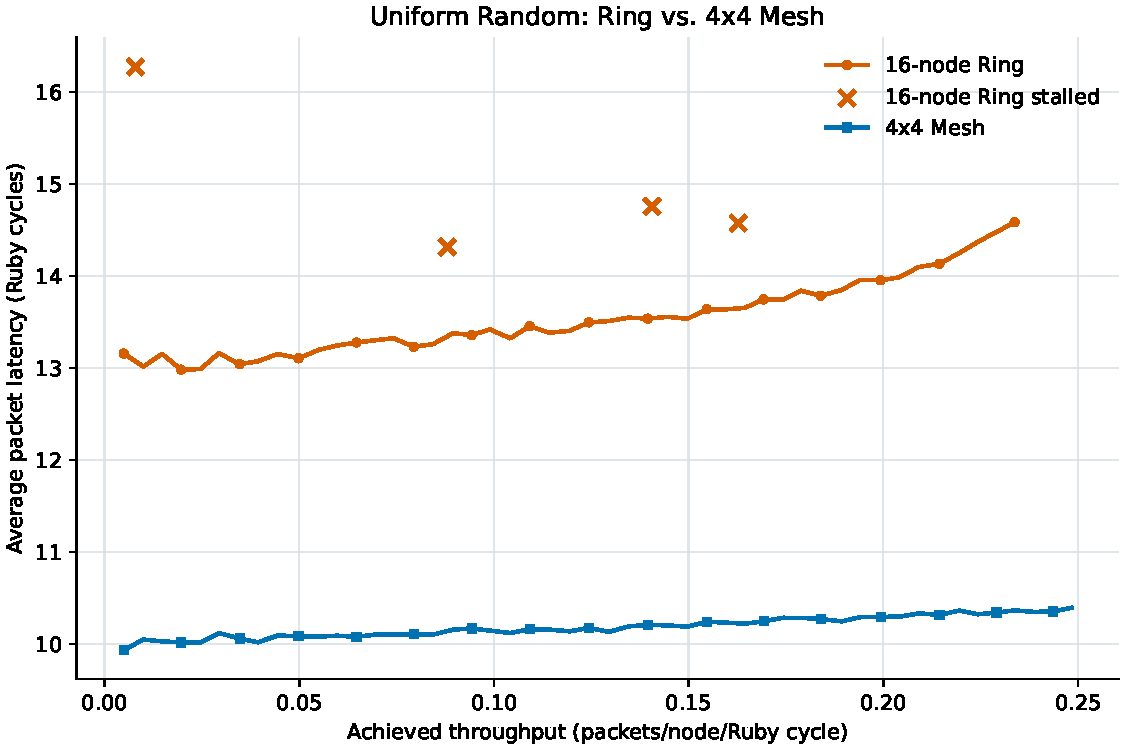
\includegraphics[width=0.94\textwidth]{../lab/lab3/task1/latency_throughput.pdf}
\caption{Task 1 latency-throughput comparison. Crosses mark points with source acceptance below 0.9.}
\label{fig:ring-latency}
\end{figure}

\begin{figure}[H]
\centering
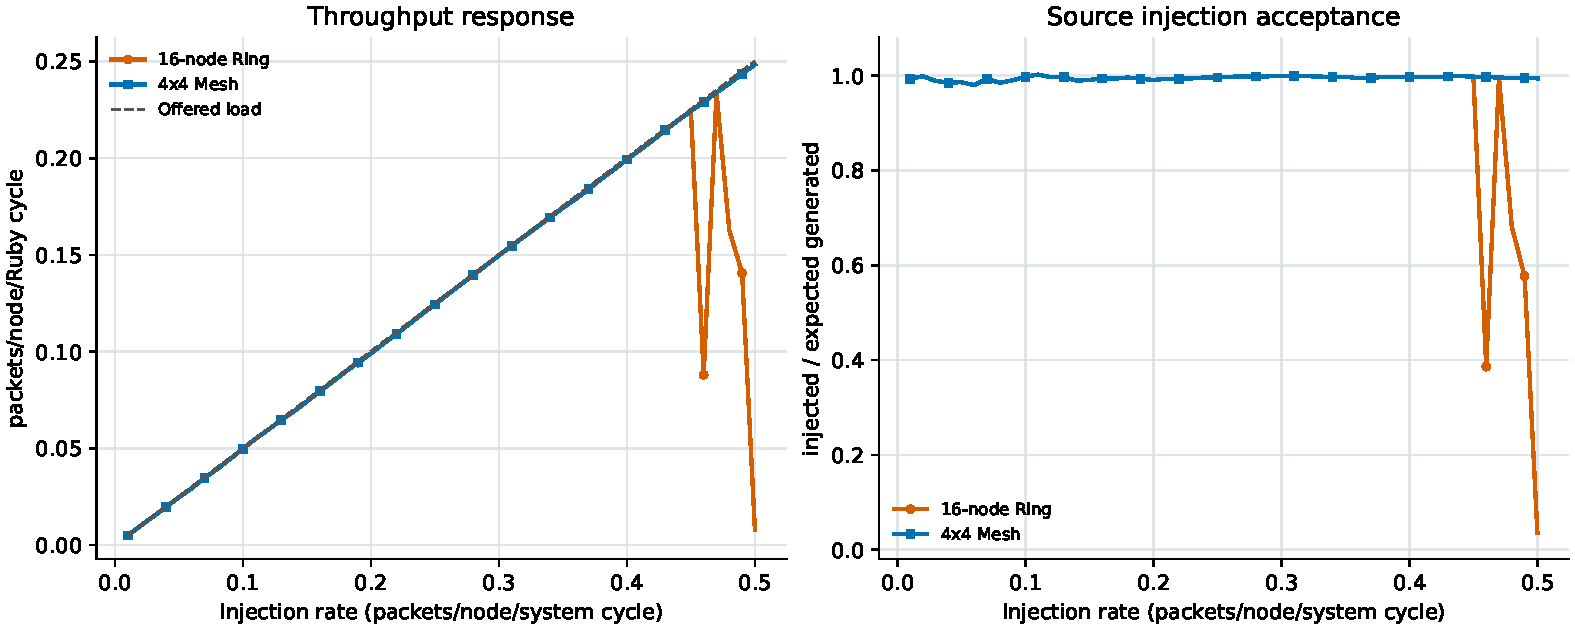
\includegraphics[width=0.98\textwidth]{../lab/lab3/task1/injection_response.pdf}
\caption{Task 1 throughput and source injection acceptance.}
\label{fig:ring-acceptance}
\end{figure}

At low load the Ring has higher latency because its average shortest path is
about four hops, compared with about 2.5 hops for the Mesh. The Ring also has
fewer independent routes and contains a cyclic channel dependency. Therefore,
near saturation, acceptance can drop sharply and later recover at an adjacent
sample: this is finite-window congestion behavior, not a claim that the Ring
has a monotonic throughput curve. The Mesh remains stable through the tested
rate of 0.50.

\section{Task 2: Wormhole Flow Control}

\subsection{Implementation}

The new \code{--wormhole} option is represented by the Garnet network
parameter \code{wormhole}. When enabled, control vnet buffers are configured
with depth 16. The implementation is intentionally limited to single-flit
\code{HEAD\_TAIL\_} packets, as required by the lab.

Normally a VC becomes idle after its tail flit and its credit is returned. In
wormhole mode, if another single-flit control packet is already queued in the
same input VC, the VC remains active, one credit is returned, and the next
packet is routed independently. Output VC selection can reuse an active VC
when it has downstream credit. The network interface similarly reuses a
control VC only when a credit is available. These changes preserve normal
packet ownership for all non-wormhole traffic.

\subsection{Comparison}

The three configurations provide the lab's requested equivalent 16-slot
comparison:

\begin{table}[H]
\centering
\small
\caption{Task 2 measured summary.}
\begin{tabular}{lrrrr}
\toprule
Configuration & Low-load latency & Max stable throughput & Max stable rate & First stalled rate \\
\midrule
VC=1, depth=1 & 13.365 & 0.039288 & 0.08 & 0.09 \\
VC=16, depth=1 & 13.158 & 0.248237 & 0.50 & not observed \\
VC=1, depth=16 (wormhole) & 13.158 & 0.248250 & 0.50 & not observed \\
\bottomrule
\end{tabular}
\end{table}

\begin{figure}[H]
\centering
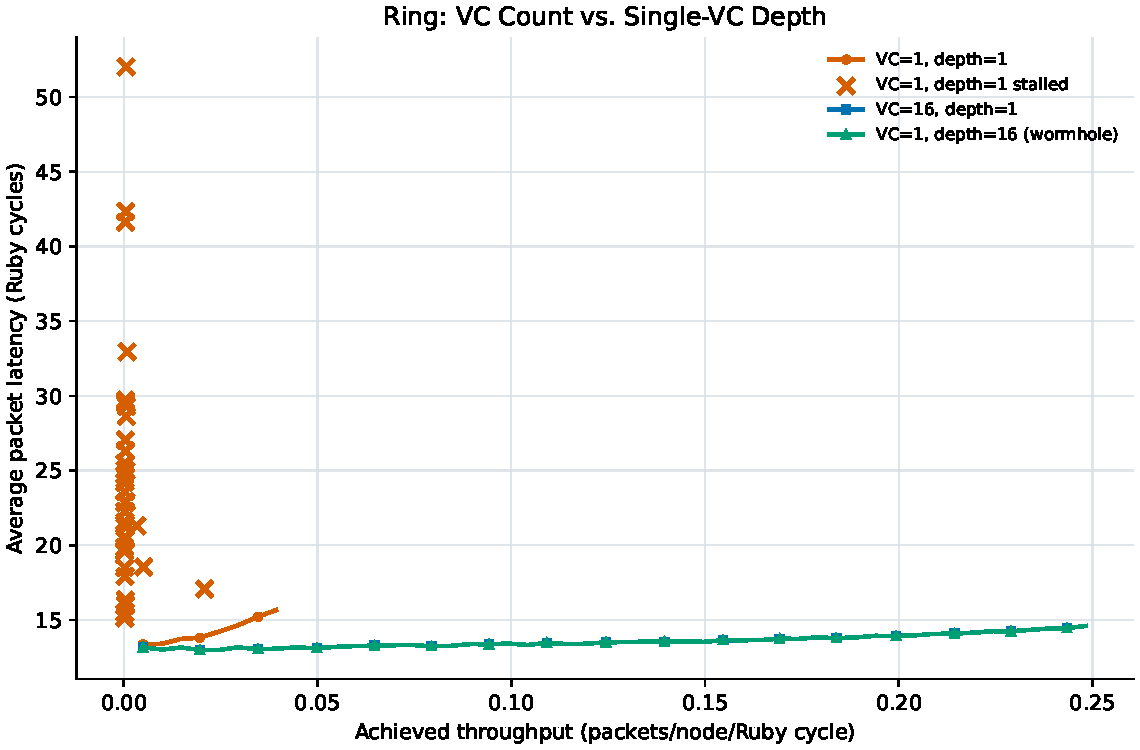
\includegraphics[width=0.94\textwidth]{../lab/lab3/task2/latency_throughput.pdf}
\caption{Task 2 latency-throughput comparison.}
\label{fig:wormhole-latency}
\end{figure}

\begin{figure}[H]
\centering
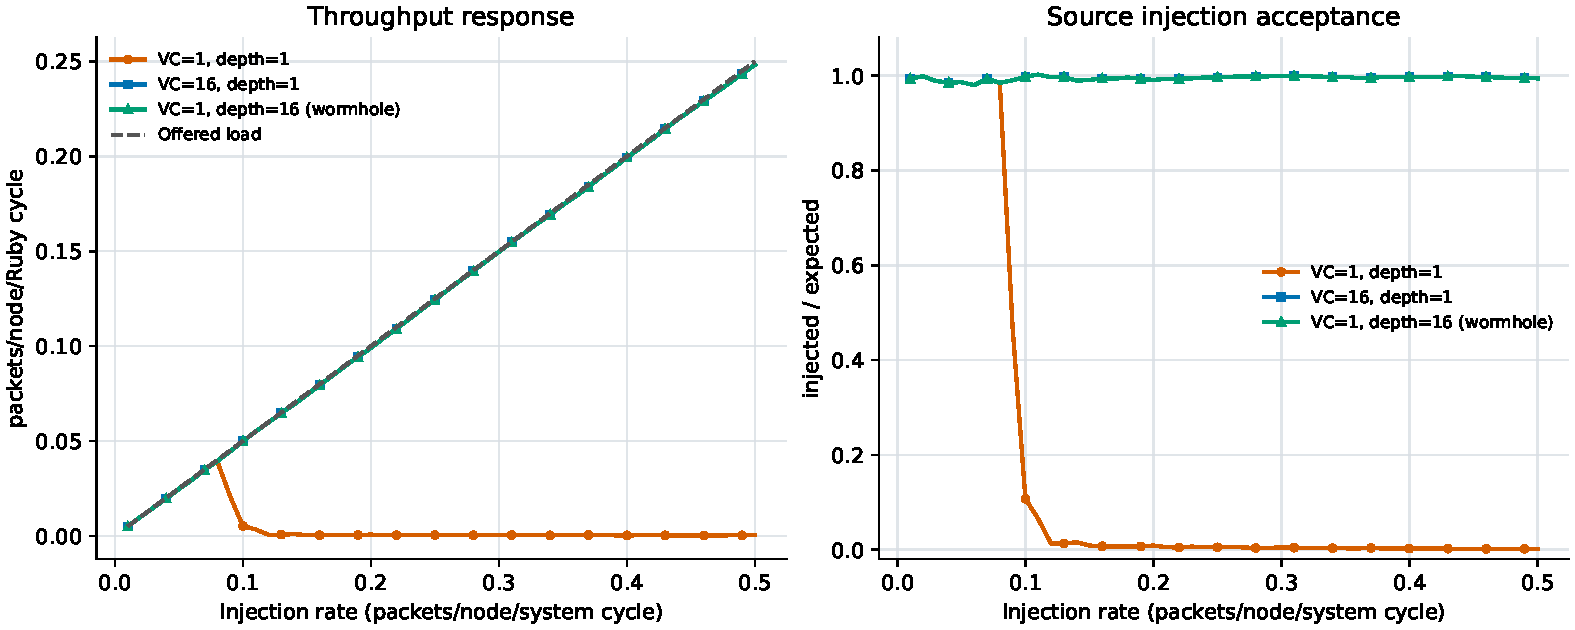
\includegraphics[width=0.98\textwidth]{../lab/lab3/task2/injection_response.pdf}
\caption{Task 2 throughput and source injection acceptance.}
\label{fig:wormhole-acceptance}
\end{figure}

With one slot, a packet must wait for the complete credit round trip before
the source can inject the next packet. This creates severe head-of-line
blocking, and the VC=1/depth=1 configuration stalls at 0.09. Sixteen VCs
provide independent routing and arbitration contexts. A single depth-16 VC
does not create more physical bandwidth; instead, it allows up to sixteen
single-flit packets to occupy the buffer while credits drain. In this
single-flit control workload, its measured throughput is essentially the same
as VC=16/depth=1.

The physical link still transmits at most one flit per cycle in every case.
The improvement comes from keeping links busy and hiding credit latency, not
from increasing link width or link rate. For multi-flit packets, a deeper
single VC could still suffer head-of-line blocking, so this result should not
be generalized beyond the specified single-flit workload.

\section{Conclusion}

The implementation satisfies both Task 1 and Task 2. The Ring topology and
custom shortest-path routing work for directed and synthetic traffic. Its
longer paths and cyclic resource dependencies explain the higher low-load
latency and high-load stalls relative to the Mesh. The wormhole mode correctly
permits multiple queued single-flit control packets in one VC. Under the
tested workload, buffer capacity is the dominant difference: one slot is
insufficient, while either sixteen independent VCs or one depth-16 wormhole
VC reaches the physical network's throughput limit.

\end{document}
